% Created 2016-05-11 Wed 23:18
\documentclass[a4paper]{article}
\usepackage[utf8]{inputenc}
\usepackage[T1]{fontenc}
\usepackage{fixltx2e}
\usepackage{graphicx}
\usepackage{grffile}
\usepackage{longtable}
\usepackage{wrapfig}
\usepackage{rotating}
\usepackage[normalem]{ulem}
\usepackage{amsmath}
\usepackage{textcomp}
\usepackage{amssymb}
\usepackage{capt-of}
\usepackage{hyperref}
\usepackage{amssymb,amsmath}
\usepackage{natbib}
\usepackage[margin=2cm]{geometry}
\usepackage{fancyhdr} %For headers and footers
\pagestyle{fancy} %For headers and footers
\usepackage{lastpage} %For getting page x of y
\usepackage{float} %Allows the figures to be positioned and formatted nicely
\floatstyle{boxed} %using this
\restylefloat{figure} %and this command
\usepackage{url} %Formatting of yrls
\rhead{
\includegraphics[width=3cm]{berkeley}}
\chead{}
\lfoot{Draft}
\cfoot{}
\rfoot{\thepage\ of \pageref{LastPage}}
\author{Peter Tittmann, Ph.D.}
\date{\today}
\title{Emissions reductions from harvested wood products and management residuals}
\hypersetup{
 pdfauthor={Peter Tittmann, Ph.D.},
 pdftitle={Emissions reductions from harvested wood products and management residuals},
 pdfkeywords={},
 pdfsubject={},
 pdfcreator={Emacs 24.5.1 (Org mode 8.3.4)},
 pdflang={English}}
\begin{document}

\maketitle
\tableofcontents

\pagebreak
\section{California forest management emissions profile}
\label{sec:orgheadline13}

\subsection{Introduction}
\label{sec:orgheadline2}

Utilization of wood biomass produced from forest management has
potential to reduce greenhouse gas (GHG) emissions and other climate
pollutants.  Currently the majority of biomass produced from forest
management activities is either left in the woods to decompose or
aggregated at a landing where it is piled and eventually burned. Woody
material resulting from a history of fire suppression, and residual
material from management activities has lead to accumulation of dead
woody material in excess of historic reference conditions and has
resulted in elevated risk of damaging wildfire in much of California's
forestland.  Prescribed natural fire and sanitation pile burning have
evolved as common practice for fuel load management in California’s
forests. However, air quality impacts of these common forestry practices as well as the opportunity cost of not using residual biomass in bioenergy energy and/or other applications weigh in favor of alternative utilization strategies. As demonstrated by  previous studies, prescribed natural fire is often only an effective tool for reducing fuel loading and maintaining fire-resilient landscapes when coupled with mechanical treatment to remove biomass (Stephens et al 2009), and open burning can be a substantial source of strong radiative forcing agents (black carbon) and criteria air pollutants (PM, NOX) when compared to use in controlled combustion biomass power plants with modern emissions control technology.

Forest management activities in California produce logs for
lumber markets and as well as maintain and enhance forest health.
In adition to merchantable logs, management activities produce logging residuals and slash that are either left
in the stand to decompose or piled and burned as directed by forest
practice rules (\href{http://calfire.ca.gov/resource_mgt/downloads/2013_FP_Rulebook_with_Tech_RuleNo1.pdf}{California Forest Practice Rules}, Article 7 §
917.2). Combustion or decomposition of this residual material results
in emissions of greenhouse gases (GHG), criteria air pollutants (CAP) and
short-lived climate pollutants (SLCP).

\begin{figure}[htb]
\centering
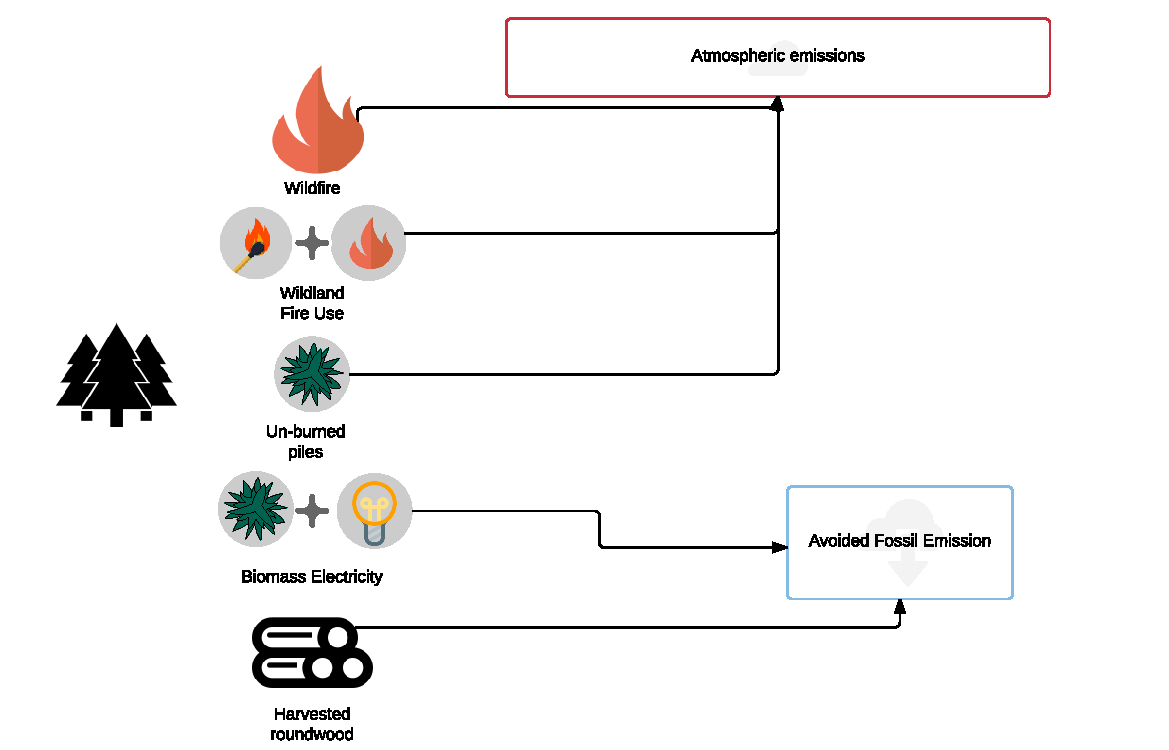
\includegraphics[width=0.75\textwidth]{./graphics/wood_fates.pdf}
\caption{Overview of the system. \label{fig:wood_fates}}
\end{figure}


Quantifying the climate effects of wood products and forest management residuals is
important to the development of the Forest Climate Plan (FCP)\footnote{The \href{http://www.fire.ca.gov/fcat/}{Forest Climate Action Team} (FCAT) was assembled in August of 2014 with the primary purpose of developing a Forest Carbon Plan by the end of 2016. FCAT is comprised of Executive level members from many of the State’s natural resources agencies, state and federal forest land managers, and other key partners directly or indirectly involved in California forestry. FCAT is under the leadership of CAL FIRE, Cal-EPA, and The Natural Resources Agency.} as well
as efforts underway by the California Board of Forestry and CalFire to
meet the intent of AB 1504 (2010). To inform these efforts, this
report provides estimates of the following :

\begin{enumerate}
\item GHG and SLCP emissions produced from the combustion or
decomposition of logging residuals.
\item GHG emissions reductions from the use of wood products harvested in
the state.
\end{enumerate}

Estimates are based on empirical data and reflect past forest
management activities. It is \textbf{critical} to note that the empirical
data used in this analysis reflect point-in-time measures that are
affected by a dynamic system of climate, growth, and mortality in
forests as well as macroeconomic and policy forces. To effective
manage forests for climate (and/or other) benefits, a process modeling
approach is necessary. This analysis may provide insight into
opportunities to more effectively utilize woody biomass residuals from
current forest management activities based on available historical
data.

Several steps are necessary to address the objective stated:

\begin{enumerate}
\item Estimate CO2 equivalent emissions from burning forest management
residuals using criteria pollutant and GHG emissions inventory
published by the California Air Resources Board (CARB)

\item Estimate the volume and fate of wood removed, left in the
forest, and burned as a result of direct anthropogenic management
activities.

\item Establish life-cycle displacement factors (DF) for all
utilized wood and apply DF to harvested wood to obtain an aggregate estimate.
\end{enumerate}

\subsubsection{Key Findings}
\label{sec:orgheadline1}

\begin{itemize}
\item Baseline emissions of GHG and SLCP emissions from burning of forest
management residuals can be estimated and should be considered in
any forest management emissions baseline.

\item Total emissions from pile burning of foreat management resulals
includine SLCP and GHG components extrapolated from CARB emissions
inventory is XXX MTCO2e

\item Harvested wood in California in 2012 resulted in avoided emissions of
4 MMTCO2e

\item Logging residuals not used in bioenergy production contributed
emissions of:
\begin{itemize}
\item XXX MMTCO2e resulting from anthropogenic burning of logging residuals

\item XXX MMTCO2e resulting from decomposition of loggin residuals left
unburned
\end{itemize}

\item Un-utilized slash from non-commercial management activities on
National Forest System lands contributed emissions of XXX MMTCO2e

\item Forest Inventory and Analysis re-sample data has been used in the
southeast to quantify removals resulting from non-commercial
management activity and could be used for this purpose in California

\item The \href{https://ssl.arb.ca.gov/pfirs/}{Prescribed Fire Information Reporting System} (PFIRS) may be a usefull tool in quantifying
emissions from pile burns and prescribed fire. However, at this time
it is not a requirement for California Air Quality Management
Districts to report emissions through this system, and thus it is not
comprehensive. It is a requirment that prescribed fires and pile
burns on National Forest System Lands are reported through PFIRS. It
is not possible at this point to associate burns in PFIRS with
commercial harvest activities.
\end{itemize}


\subsection{Estimating CO2 equivalent emissions from forest biomass burning}
\label{sec:orgheadline4}

\begin{figure}[htb]
\centering
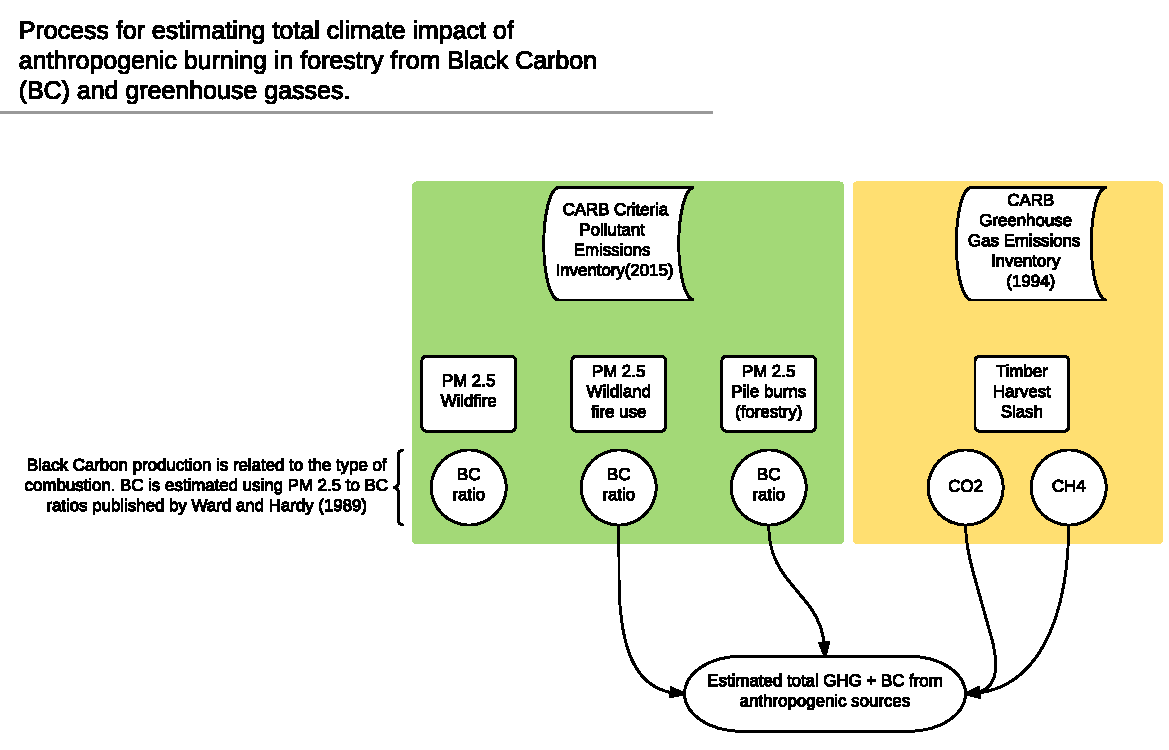
\includegraphics[width=0.75\textwidth]{./graphics/burning.pdf}
\caption{Data sources available from CARB for estimating GHG and SLCP emissions from forest management. \label{fig:wood_fates}}
\end{figure}


\subsubsection{Estimating black carbon emissions from biomass burning}
\label{sec:orgheadline3}

The California Air Resources Board (CARB) reports
emissions from forest biomass burning  in the most current
\href{http://www.arb.ca.gov/ei/ei.htm}{statewide emissions inventory}. The Criteria Air
Pollutant (CAP) emissions inventory and the Greenhouse Gas (GHG)
emissions inventory are both necessary sources for establishing
aggregate annual climate-forcing emissions. The GHG inventory captures
gasses with radiative forcing properties but does not capture elemental
carbon or black carbon (BC) emissions which have strong radiative
forcing properties. The \citet{CaliforniaAirResourcesBoard2015,CaliforniaAirResourcesBoard2016}
reports aggregate SLCP emissions from wildfire
(\texttt{80.52} MMTCO2e), and from prescribed fire
(\texttt{3.66} MMTCO2e). However, no reference in the
SLCP Strategy is made to the source of these estimates.

The California Air Resources Board has published
\href{http://www.arb.ca.gov/ei/emissiondata.htm}{criteria air pollutant
emissions estimates for 2015}. Particulate matter as reported in the
criteria air pollutant emissions inventory contains black carbon which
is a strong short lived climate pollutant.


\begin{table}[htb]
\centering
\begin{tabular}{rrrrrrl}
GWP\(_{\text{20}}\) & GWP\(\sigma_{\text{20}}\) & GWP\(_{\text{100}}\) & GWP\(\sigma_{\text{100}}\) & GWP\(_{\text{500}}\) & GWP\(\sigma_{\text{500}}\) & Source\\
\hline
2200.0 & 888.82 & 633.33 & 255.41 & 193.33 & 77.67 & Fuglestvedt2010\\
3200.0 &  & 900.0 &  &  &  & CaliforniaAirResourcesBoard2015\\
\end{tabular}
\caption{Range of GWP values for Black Carbon.}

\end{table}




CARB reports PM 2.5 emissions in tons/day. Annual emissions  as
reported by CARB are shown in

\begin{center}
\begin{tabular}{lr}
Source & PM 2.5 (t y\(^{\text{-1}}\))\\
\hline
ALL VEGETATION & 137630.15\\
FOREST MANAGEMENT & 5480.51\\
WILDLAND FIRE USE (WFU) & 6802.43\\
\end{tabular}

\end{center}

Black Carbon emissions
can be estimated from PM 2.5 emissions if the ratio of smoldering to
flaming combustion is known. \citet{Ward1989} provide estimates of
the ratio of smoldering to flaming combustion for a hand/machine piled
burns, prescribed natural fire and wildfire. BC is a fraction
of the Total Carbon (TC) component of PM 2.5. Thus BC is related to PM
2.5 by Eq. \eqref{eq-bc} :



\begin{align}
BC &= \left( PM_{2.5} \times F \times TC_f \times BC_f\right) + \left( PM_{2.5} \times S \times TC_s \times BC_s\right) \label{eq-bc} \\
\text{where:} \nonumber \\
BC &= \text{Black Carbon (mass units)} \nonumber \\
PM_{2.5} &= PM_{2.5} \text{ (mass units)} \nonumber \\
F &= \text{Percent of combustion in flaming phase} \nonumber \\
TC_f &= \text{Total Carbon fraction of } PM_{2.5} \text{ for flaming phase} \nonumber \\
BC_f &= \text{Black Carbon fraction of Total Carbon for flaming phase} \nonumber \\
S &= \text{Percent of combustion in smoldering phase} \nonumber \\
TC_s &= \text{Total Carbon fraction of } PM_{2.5} \text{ for smoldering phase} \nonumber \\
BC_s &= \text{Black Carbon fraction of Total Carbon for smoldering phase} \nonumber
\end{align}

Based on \citet{Ward1989} and \citet{Jenk1996} the following ratios are
used herein.

\begin{table}[htb]
\centering
\begin{tabular}{lrrrrrr}
Source & BC\(_{\text{f}}\) t\(^{\text{-1}}\) PM & TC\(_{\text{f}}^{\text{Cv}}\) t\(^{\text{-1}}\) PM & BC\(_{\text{f}}^{\text{Cv}}\) t\(^{\text{-1}}\) TC & BC\(_{\text{s}}\) t\(^{\text{-1}}\) PM 2.5 & TC\(_{\text{s}}^{\text{Cv}}\) t\(^{\text{-1}}\) PM & BC\(_{\text{s}}^{\text{Cv}}\) t\(^{\text{-1}}\) TC\\
\hline
Pile Burn & 0.046904 & 0.09 & 0.45 & 0.01624 & 0.01 & 0.49\\
Prescribed & 0.08016309 & 0.0733 & 0.5833 & 0.020944 & 0.08 & 0.29\\
Wildfire & 0.05870124 & 0.0867 & 0.4467 & 0.0228641 & 0.06 & 0.338\\
\end{tabular}
\caption{Factors used for calculating Black Carbon (BC) emissions from three primary combustion sources. BC is a fraction of Total Carbon (TC) which is a fraction of total PM 2.5. Coefficients of variation (C\(_{\text{v}}\)) are reported here as well.}

\end{table}



To arrive at a rough estimate of BC emissions based on PM2.5 the
following steps are taken

\begin{enumerate}
\item Determine the amount of PM2.5 produced in the flaming and smoldering
phases of combustion for each type (piles, prescribed,
wildfire). Ratios from \citet{Ward1989}, table 5 are used.
\item Define 1000 normal probability distributions using the coefficient
of variation from Table \ref{tab:bc_pmfor} the percent of PM2.5
comprised of carbonaceous material (TC) and percent of TC comprised
of black carbon (BC) give estimates and coefficient of variation
estimates provided by \citet{Ward1989}, tables 2 and 3.
\item Estimate annual BC emissions based on probability distributions
defined in 2.
\end{enumerate}

The following plot represents estimates of total BC emissions resulting
from combustion of biomass in the CARB CPE emissions categories
reflecting woody biomass combustion in wildfire, pile burning and
prescribed natural fire.

\begin{figure}[htb]
\centering
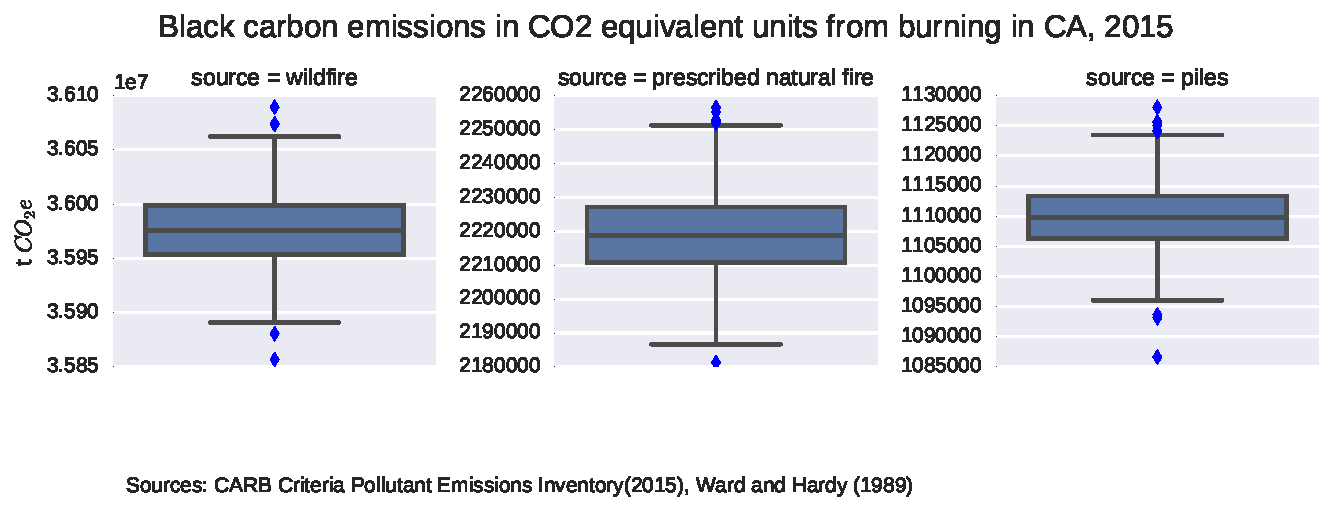
\includegraphics[width=\textwidth]{./graphics/bc_prob_gwp.pdf}
\caption{Short-lived climate pollution from open burning of biomass as reported by CARB criteria pollutant emissions inventory.}
\end{figure}

In addition the
\url{http://www.arb.ca.gov/cc/inventory/archive/tables/net_co2_flux_2007-11-19.pdf}
CARB 1994 greenhouse gas emissions inventory estimates emissions from
wildfire and slash burning through 2004 (Table \ref{arb_ghg_2004}).
\begin{center}
\begin{tabular}{lr}
Source Category & Average annual emissions 1994-2004 MMTCO\(_{\text{2e}}\)\\
\hline
Forest and rangeland fires & 2.0194\\
Timber harvest slash & 0.155266666666667\\
\end{tabular}

\end{center}


To arrive at an estimate of total emissions in 2015 from burning forest
management residuals in CO2 equivalent terms from published CARB
estimates we can combine the CO2 emissions reported for 2004 in the
LULUC Biodegradable Carbon Emissions and Sinks with black carbon
emissions extrapolated from the CARB Criteria Air Pollutant Emissions
inventory estimates. The time discrepancy between the 2004 and 2015 is
acknowledged as an irreconcilable source of uncertainty in this
estimation. Further model based estimation could be used to derive a
ratio of GHG to PM using the CONSUME model. This does however show that a baseline of
substantial emissions from forest management residuals has been reported
in CARB emissions inventories and should be recognized as a baseline
condition. We find that a rough estimate of CO2e emissions from pile
burning annual approaches 1 Mt CO2e.

\begin{center}
\begin{tabular}{rrl}
 & Mt CO2e & Source\\
\hline
0 & 0.17 & CO2 pile burning\\
1 & 0.99 & CO2e BC pile burning\\
2 & 1.16 & Total Mt CO2e\\
\end{tabular}

\end{center}

BC emissions in terms of CO2e has not been included in any GHG emissions
inventory published by CARB.

\subsection{Climate impact of harvested wood}
\label{sec:orgheadline11}

\url{https://www.lucidchart.com/publicSegments/view/52a1774e-7722-4ebf-8e1a-e8fc6837bfee/image.png}




\subsubsection{Wood Displacement Factors}
\label{sec:orgheadline5}

Wood harvested from California's forests is used in construction,
landscaping and consumer products. In all of its applications, a range
of other products can be used in place of wood. For example, in
residential construction, precast concrete and structural steel framing
are competitive alternatives to wood. The choice of materials used in
construction has a profound impact on GHG emissions from the
construction sector. This impact can be expressed as a displacement
factor (DF). A displacement factor quantifies the amount of emissions
reduction achieved per unit of wood used. A
\href{https://docs.google.com/uc?id=0B9-9Vlx0SkkFNjVGU0NrTm9HZ3M&export=download}{meta
analysis} conducted by \citep{Sathre2010} compared empirical analysis from 21 international studies and found an
average emissions reduction of 2.1 tons of carbon (3.9 t CO2e) per ton
of dry wood used. Studies ranged substantially around the average, the
authors found that the majority of published displacement factors ranged
between 1 and 3 tC/t dry wood. The displacement factors published in
\citep{Sathre2010} and used in this analysis include the
following sources emissions reduction:

\begin{enumerate}
\item \textbf{Reduced emissions from manufacturing:} Wood products require total
energy than than manufacturing most alternative materials.
\item \textbf{Avoided process emissions:} Wood-alternatives such as cement have
substantial CO2 emissions associated with production.
\item \textbf{Carbon storage in products:} Carbon in harvest wood was drawn from
the atmosphere through photosynthesis and will remain fixed through
the useful life of the wood product.
\item \textbf{Carbon storage in forests:} Forests producing wood continue to grow.
It is assumed that forests producing wood in California are managed
to sustain forest growth (not converted to non-forest land uses).
\item \textbf{Avoided fossil fuel emissions due to bioenergy substitution:}
Logging and milling residuals used to produce energy avoid emissions
from fossil energy sources in the energy sector.
\item \textbf{Carbon dynamics in landfills:} A fraction of carbon in wood
deposited in landfills post use remains in semi-permanent storage.
The remainder is converted to methane through biological
decomposition in the landfill. Capture and use of the methane as an
energy source, in turn reduces emissions from fossil energy sources.
\end{enumerate}

\subsubsection{Displacement Factors Applied to Timber Products Output}
\label{sec:orgheadline6}

To evaluate the climate impact of harvested wood in California I use
harvested roundwood estimates from the
\href{http://srsfia2.fs.fed.us/php/tpo_2009/tpo_rpa_int1.php}{Timber
Products Output (TPO)} database. I use two estimates of the DF applied
to the harvested wood reported in the TPO based on weather logging
residuals are used in bioenergy or left in the woods to decompse or
burn.
\url{https://www.lucidchart.com/publicSegments/view/fb78eea4-7fba-4a78-8e98-25fdd66a3df2/image.png}

I use displacement factors reported by Sathre and O'Connor
(\href{https://docs.google.com/spreadsheets/d/13UQtRfNBSJ81PXxbYSnB2LrjHePNcvhJhrsxRBjHpoY/pubhtml?gid=546564075&single=true}{Table
3}) applied to the reported volumes from the TPO. The following
references are used to arrive at a displacement factor for harvested
roundwood without logging residue utilization.

\begin{center}
\begin{tabular}{lr}
reference & displacement factor\\
\hline
Eriksson et al. (2007) & 1.7\\
Eriksson et al. (2007) & 2.2\\
Salazar and Meil (2009) & 4.9\\
Werner et al. (2005) & 1.7\\
\end{tabular}

\end{center}

I use an average of the DF reported here of \textbf{2.625} tCO2e/t finished
wood product.

For harvested roundwood with logging residue utilization the following
studies are used.

\begin{center}
\begin{tabular}{lr}
reference & displacement factor\\
\hline
Eriksson et al. (2007) & 1.9\\
Eriksson et al. (2007) & 2.5\\
Gustavsson et al. (2006) & 4\\
Gustavsson et al. (2006) & 5.6\\
Gustavsson et al. (2006) & 2.2\\
Gustavsson et al. (2006) & 3.3\\
Pingoud and Perala (2000) & 3.2\\
\end{tabular}

\end{center}

I use an average of the DF reported here of \textbf{3.243} tCO2e/t finished
wood product.

TPO is reported in terms of roundwood harvested for products. The
displacement factors presented in Sathre and O'Connonr are in terms of
tons of finished wood products. Therefore we must assume a milling
efficiency to convert TPO estimates to finished wood products. I assume
a milling efficiency of 0.5.

Further, TPO is reported in in cubic feet and the DF implies a mass
unit. To convert cubic meters to a mass unit we use the average wood
density of harvested volume in California weighted by species. Harvest
volume by species is reported in McIver and Morgan
(\href{https://docs.google.com/spreadsheets/d/138FWlGeW57MKdcz2UkWxtWV4o50SZO8sduB1R6JOFp8/pubhtml?gid=393414465&single=true}{Table
4}). The resulting weighted average wood density used here is \textbf{27.94
lbs/cuft}.

McIver and Morgan report the percent of harvest used as bioenergy
feedstock. From personal communications with
\href{http://www.bber.umt.edu/staff/mciver.asp}{Chelsea McIver}, all
bioenergy feedstock reported is sourced in-woods (ie, not mill
residues).

\begin{center}
\begin{tabular}{rrr}
 & year & bioenergy \% of harvest\\
\hline
0 & 2000 & 0.024\\
1 & 2006 & 0.036\\
2 & 2012 & 0.082\\
\end{tabular}

\end{center}

The TPO reports the total logging residues produced from the states
harvest.

\begin{center}
\begin{tabular}{rlrrr}
 & Ownership & Roundwood Products & Logging Residues & Year\\
\hline
0 & National Forest & 72.4 & 20.7 & 2012\\
1 & Other Public & 16.2 & 3.4 & 2012\\
2 & Forest Industry & 328.9 & 72.4 & 2012\\
3 & Other Private & 53 & 11.2 & 2012\\
4 & National Forest & 52.8 & 16.3 & 2006\\
5 & Other Public & 1.1 & 0.3 & 2006\\
6 & Forest Industry & 274.3 & 59.6 & 2006\\
7 & Other Private & 139.2 & 33.2 & 2006\\
8 & National Forest & 90.8 & 22.6 & 2000\\
9 & Other Public & 5.2 & 1.6 & 2000\\
10 & Forest Industry & 372.5 & 70.6 & 2000\\
11 & Other Private & 159.4 & 49.1 & 2000\\
12 & National Forest & 132.1 & 11.2 & 1994\\
13 & Other Public & 24.7 & 4.3 & 1994\\
14 & Forest Industry & 396.1 & 63.1 & 1994\\
15 & Other Private & 174.7 & 22.3 & 1994\\
\end{tabular}

\end{center}

The ratio of harvested volume to which we can apply a displacement
factor reflecting bioenergy use of logging residuals can be calculated
based on the ratio of reported consumption of logging residuals in
bioenergy by McIver and Morgan to the total logging residuals reported
in the TPO. McIver and Morgan report bioenergy consumption from 2000
forward. For years previous, we use the average bioenergy consumption
from 2000 -- 2012.

To calculate the total emissions reduction resulting from California's
timber harvest, we apply the appropriate displacement factor (with or
without logging residual utilization) to the commensurate fraction of
harvested roundwood. The results are shown in the following chart.

\url{https://raw.githubusercontent.com/peteWT/fcat_biomass/master/graphics/harv_em_reductions.png}
\subsubsection{Emissions from un-utilized logging residues}
\label{sec:orgheadline8}

From logging residuals not used in bioenergy, emmisions are produced
from combustion of the residual material or from decomposition of the
material over time. To calculate the ratio of burned to decompsed
logging residues I begin with the CARB estimate of PM2.5 produced from
forest management. \#\#\#\# Estimate biomass from PM2.5 To estimate total
biomass from PM2.5 I assume 90\% consumption of biomass in piles and use
the relationship of pile tonnage to PM emissions calculated using the
\href{http://depts.washington.edu/nwfire/piles/}{Piled Fuels Biomass and
Emissions Calculator} provided by the Washington State Department of
Natural Resources. This calculator is based on the
\href{http://www.fs.fed.us/pnw/fera/research/smoke/consume/index.shtml}{Consume}
fire behavior model published by the US Forest Service.

\begin{center}
\begin{tabular}{rrlrr}
 & YEAR & EICSOUN & Annual PM 2.5(t) & Biomass (BDT)\\
\hline
0 & 2000 & FOREST MANAGEMENT & 5474.31 & 901120\\
1 & 2005 & FOREST MANAGEMENT & 5474.31 & 901120\\
2 & 2010 & FOREST MANAGEMENT & 5474.31 & 901120\\
3 & 2012 & FOREST MANAGEMENT & 5477.3 & 901613\\
4 & 2015 & FOREST MANAGEMENT & 5480.51 & 902142\\
\end{tabular}

\end{center}

Total emissions resulting from pile burned forest management residuals
can then be derived for the two greenhouse gasses produced from pile
burning (CO2, CH4) and from BCn:

\begin{center}
\begin{tabular}{rrlrrrr}
 & Year & Emissions source & CO2 (t) & CH4 (tCO2e) & BC (tCO2e) & Pile Burn Total (tCO2e)\\
\hline
0 & 2000 & FOREST MANAGEMENT & 1.34928\,(+06) & 127280 & 248255 & 1.72481\,(+06)\\
1 & 2005 & FOREST MANAGEMENT & 1.34928\,(+06) & 127280 & 248255 & 1.72481\,(+06)\\
2 & 2010 & FOREST MANAGEMENT & 1.34928\,(+06) & 127280 & 248255 & 1.72481\,(+06)\\
3 & 2012 & FOREST MANAGEMENT & 1.35002\,(+06) & 127349 & 248391 & 1.72576\,(+06)\\
4 & 2015 & FOREST MANAGEMENT & 1.35081\,(+06) & 127424 & 248536 & 1.72677\,(+06)\\
\end{tabular}

\end{center}

\begin{enumerate}
\item Emissions from decomposition of un-utilized forest management
\label{sec:orgheadline7}
residuals

Un-utilized residual biomass not consumed in pile burns decomposes over
time resulting in emission of methane and carbon dioxide. To provide a
full picture of the emissions from residual material produced from
commercial timber harvesting in California, decomposition of unutilized
logging residuals left on-site that are not burned must be accounted
for. To establish the fraction of logging residue that is left to
decompose, residues burned and used in bioenergy are subtracted from the
total reported by the TPO: \url{http://mathurl.com/h5ns5j4.png}

To calculate the GHG emissions from decomposition of piles we use the
following equation:

\url{http://mathurl.com/jzspdak.png}
\end{enumerate}
\subsubsection{Emissions from non-commercial management residuals}
\label{sec:orgheadline10}

/Note: Residues from non-commercial management activities are assumed to
be small in comparison with logging residues. In addition, there is
presently no empirical data available. As such, estimating these volumes
has not been prioritied. I have attempted to provide an estimate for
public lands in the National Forest System./

The TPO in California does not report wood volume produced from
non-commercial management activities. This includes management
activities such as pre-commercial thinning, sanitation thinning, and
fuels reduction thinning. To estimate the volume of material produced
from these activities we use the following sources:

\begin{enumerate}
\item \textbf{Public lands:} The USFS Forest Service Activity Tracking System
(FACTS) reports management activities conducted on National Forest
System Lands. To ensure estimates of biomass volume using FACTS are
not duplicative of reported volume in the TPO a series of filters are
applied to the FACTS attributes to identify only non-commercial
management activities.
\item \textbf{Private industrial timber lands:} CalFIRE's
\href{http://www.calfire.ca.gov/resource_mgt/resource_mgt_forestpractice_gis}{Forest
Practice Geographical Information System}. \textbf{TODO}
\end{enumerate}

\begin{enumerate}
\item Forest Service Activity Tracking System (FACTS)
\label{sec:orgheadline9}

Data from TPO does not account for forest management activities that do
not result in commercial products (timber sales, biomass sales). The
USFS
\href{http://data.fs.usda.gov/geodata/edw/datasets.php?dsetParent=Activities}{reports}
Hazardous Fuels Treatment (HFT) activities as well as Timber Sales (TS)
derived from the FACTS database. I use these two data sets to estimate
the number of acres treated that did not produce commercial material
(sawlogs or biomass) and where burning was not used. The first step is
to eliminate all treatments in the HFT data set that included timber
sales. I accomplish this by eliminating all rows in the HFT data set
that have identical \texttt{FACTS\_ID} fields in the TS dataset. I further
filter the HFT dataset by removing any planned but not executed
treatments (\texttt{nbr\_units1 >0} below -- \texttt{nbr\_units1} references
\texttt{NBR\_UNITS\_ACCOMPLISHED} in the USFS dataset, see metadata for HFT
\href{http://data.fs.usda.gov/geodata/edw/edw_resources/meta/S_USA.Activity_HazFuelTrt_PL.xml}{here}),
and use text matching in the 'ACTIVITY' and 'METHOD' fields to remove
any rows that contain reference to 'burning' or 'fire'. Finally, we
remove all rows that that reference 'Biomass' in the method category as
it is assumed that this means material was removed for bioenergy.I use a
range of 10-35 BDT/acre to convert acres reported in FACTS to volume.
The following table presents descriptive statistics for estimates of
residual unutilized wood biomass on an annual basis in million cubic
feet.

\begin{center}
\begin{tabular}{lrrrrr}
 & nf$\backslash$\(_{\text{ncmr}}\) & nf$\backslash$\(_{\text{lr}}\) & opriv$\backslash$\(_{\text{lr}}\) & fi$\backslash$\(_{\text{lr}}\) & opub$\backslash$\(_{\text{lr}}\)\\
\hline
count & 11 & 4 & 4 & 4 & 4\\
mean & 12.0194 & 17.7 & 28.95 & 66.425 & 2.4\\
std & 4.68948 & 5.07346 & 16.1593 & 6.07639 & 1.79444\\
min & 2.37421 & 11.2 & 11.2 & 59.6 & 0.3\\
25\% & 8.92407 & 15.025 & 19.525 & 62.225 & 1.275\\
50\% & 13.3557 & 18.5 & 27.75 & 66.85 & 2.5\\
75\% & 14.5349 & 21.175 & 37.175 & 71.05 & 3.625\\
max & 17.8532 & 22.6 & 49.1 & 72.4 & 4.3\\
\end{tabular}

\end{center}

\textbf{TODO} - [x] Public lands non-commercial management residuals - [ ]
Private land non-commercial management residuals - [x] Public lands
logging residuals - [x] Private lands logging residuals
\end{enumerate}

\subsection{References}
\label{sec:orgheadline12}

Ward DE, Hardy CC. Organic and elemental profiles for smoke from
   prescribed fires. In: Watson JG, editor. International specialty
   conference of the Air and Waste Management Association
   [Internet].San Francisco: Air and Waste Management
   Association; 1989. Available from:
   \url{https://docs.google.com/uc?id=0B9-9Vlx0SkkFaU1ITkFjQnBXUEk&export=download}

Jenkins BM, Turn SQ, Williams RB, Goronea M, Abd-el-Fattah H,
   Mehlschau J, et al. Atmospheric Pollutant Emissions Factors From Open
   Burning of Agricultural and Forest Biomass By Wind Tunnel Simulations
   [Internet]. Sacramento, CA; 1996. Available
   \href{https://docs.google.com/uc?id=0B9-9Vlx0SkkFN1dQVjFkOXI1eVE&export=download}{here}

Mciver CP, Meek JP, Scudder MG, Sorenson CB, Morgan TA, Christensen GA.
California's Forest Products Industry and Timber Harvest. Portland, OR;
\begin{enumerate}
\item
\end{enumerate}
\url{https://docs.google.com/uc?id=0B9-9Vlx0SkkFRHk5c2czeFR2WTQ&export=download}

Sathre R, O'Connor J. Meta-analysis of greenhouse gas displacement
factors of wood product substitution. Environ Sci Policy [Internet].
2010 Apr;13(2):104--14. Available from:
\url{https://docs.google.com/uc?id=0B9-9Vlx0SkkFNjVGU0NrTm9HZ3M&export=download}

Gustavsson L, Pingoud K, Sathre R. Carbon Dioxide Balance of Wood
Substitution: Comparing Concrete- and Wood-Framed Buildings. Mitig Adapt
Strateg Glob Chang [Internet]. 2006 May;11(3):667--91. Available from:
\url{https://docs.google.com/uc?id=0B9-9Vlx0SkkFMS1Jb2VwV2FfR2M&export=download}

Eriksson E, Gillespie AR, Gustavsson L, Langvall O, Olsson M, Sathre R,
et al. Integrated carbon analysis of forest management practices and
wood substitution. Can J For Res [Internet]. 2007 Mar;37(3):671--81.
Available from:
\url{https://docs.google.com/uc?id=0B9-9Vlx0SkkFcEduQUozRzVja28&export=download}

Pingoud K, Perälä A, Pussinen A. Carbon dynamics in wood products. Mitig
Adapt Strateg Glob Chang [Internet]. 2001;6(2):91--111. Available from:
\url{http://link.springer.com/article/10.1023/A:1011353806845}

Salazar J, Meil J. Prospects for carbon-neutral housing: the influence
of greater wood use on the carbon footprint of a single-family
residence. J Clean Prod [Internet]. 2009 Nov;17(17):1563--71. Available
from:
\url{https://docs.google.com/uc?id=0B9-9Vlx0SkkFQTByZEU1eWtHZWs&export=download}
Table xxx: HWP pools (Thousand Tons of C02e)

\bibliographystyle{IEEEtranSN}
\bibliography{fcat}
\end{document}